\documentclass[12 pt]{article}
\usepackage{amsmath,amsfonts,parskip}
\usepackage[a4paper]{geometry}
\usepackage[T1]{fontenc}
\usepackage{enumerate}
\usepackage{graphicx}

\begin{document}

\begin{center}
       \large{
       \textbf{Computational Physics - PH3264} \break
	Assignment 1
}
\end{center}

\textbf{Krishna Iyer V S \hfill Roll:20201017}
\hrule 
\vspace{0.1cm}

\begin{enumerate}[a.]

\item
For a-f, refer to respective .cpp and .out files for demonstration - all involve printing random numbers with different seeds, and other simple tasks.

\setcounter{enumi}{6}

\item
The output from g.out is as follows:
\begin{verbatim}
Absolute difference between 0.5 and average of random numbers
10        : 0.1838132364
100       : 0.02390399648
10000     : 0.0004469846813
1000000   : 5.272165292e-05
\end{verbatim}
The expected value is 0 (as the number of random numbers sampled tends to infinity, the average approaces 0.5). As the number of sample here increases, the difference gets closer to 0 - verifying the law of large numbers.

\item
The following plot shows the distribution of the sum of 10000 random numbers, computed 10000 times.

\begin{figure}[htb!]
\centering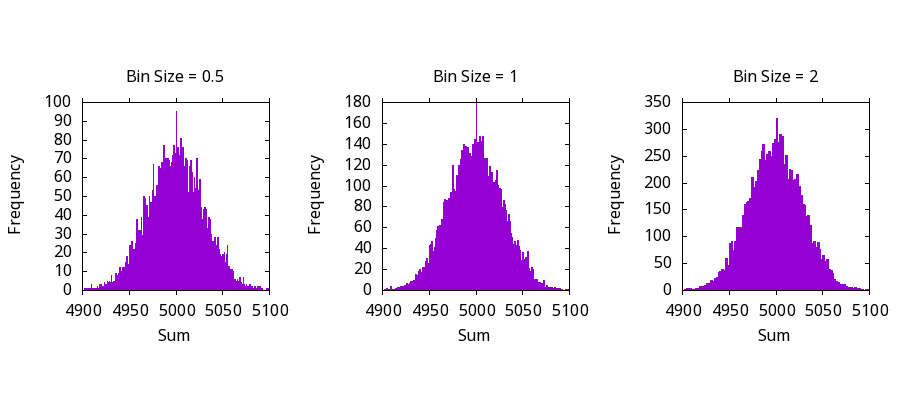
\includegraphics[width=6.0in]{plots/random_numbers_sum.png}
\end{figure}

\item
While it is not clear from the plot shown, zooming in shows that the bars alternate - this is because the sum of 10000 odd numbers (-1 and 1) is always even, causign the values for the bins (2n,2n+1) to be 0.
\pagebreak
\begin{figure}[htb!]
\centering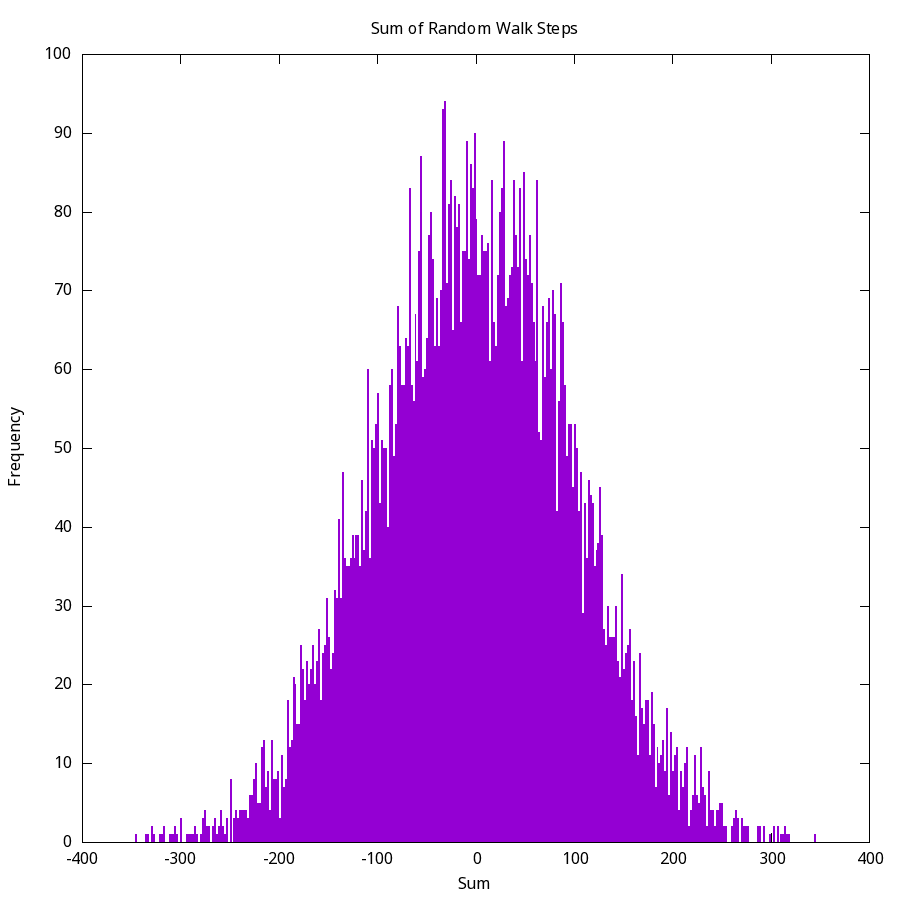
\includegraphics[width=4.5in]{plots/random_walk_sum_10e4x10e4.png}
\end{figure}

\item
The plot below shows the same distribution with various bin sizes - Histograms with larger bin sizes are smoother.
\begin{figure}[htb!]
\centering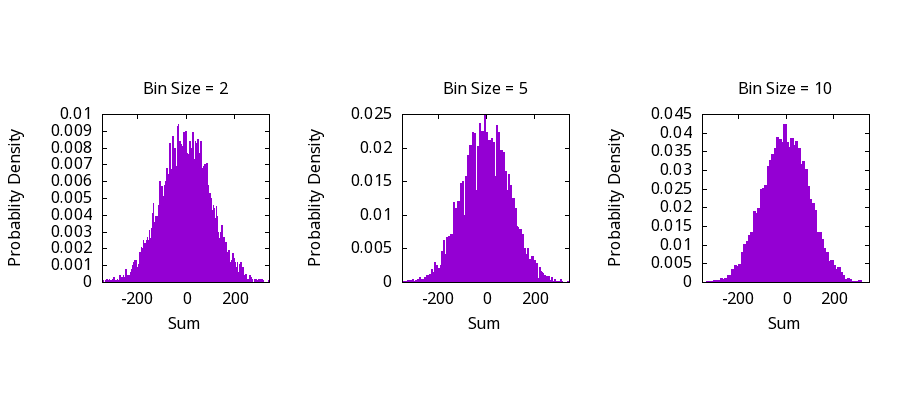
\includegraphics[width=5.6in]{plots/random_walk_sum_10e4x10e4_bins.png}
\end{figure}

Note: All plots hereafter are normalized such that the cumulative sum is 1.

\item
The plots for $10^5$ samples of sum of $10^4$ steps and $10^5$ steps are shown below, using a bin width of 2.

\item
As can be seen in the plots below, with more samples at every step, the standard deviation increases. More samples indicates more steps - with more steps in a walk, regions farther from the origin are more accessible, explaining this spread.
\begin{figure}[htb!]
\centering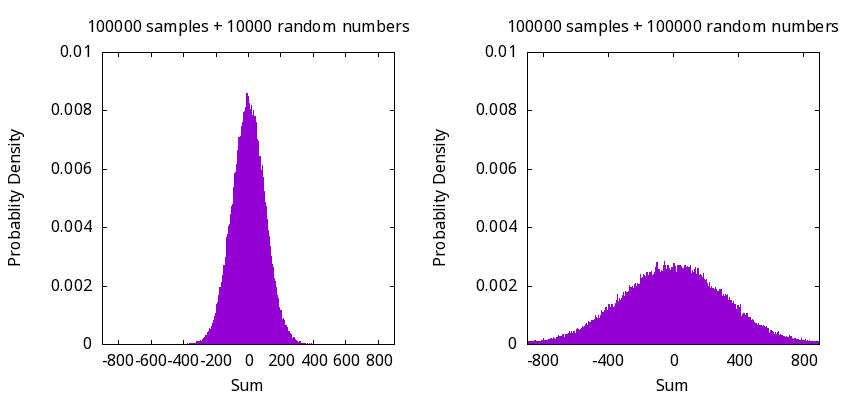
\includegraphics[width=5.5in]{plots/random_walk_sum_10e5_bins.png}
\end{figure}

\item
Shown below are the distributions with gaussian fits.(binsize=1)
\vspace{4cm}
\centering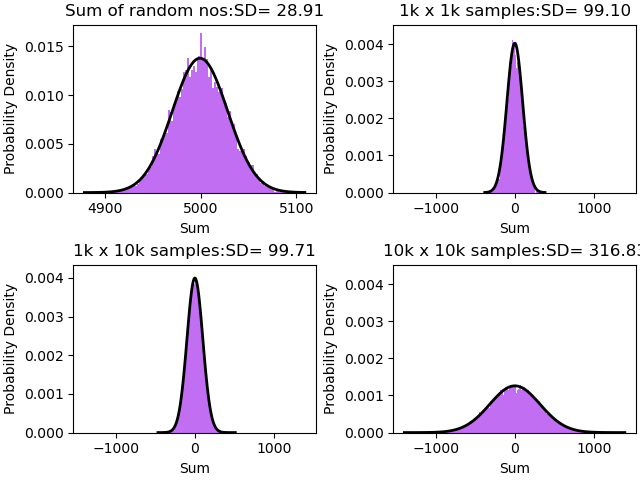
\includegraphics[width=4.8in]{plots/plots_with_fit.png}

\end{enumerate}
\end{document}
